\documentclass[dvips,xcolor=pst]{beamer}
%\documentclass[dvips,handout,xcolor=pst]{beamer}
%\documentclass[letterpaper]{article}
%\usepackage{beamerarticle}
\newcommand{\newblock}{}
\usepackage{pstricks}
%\usepackage{hyperref}
%\usepackage[authoryear]{natbib}
\usepackage{graphicx}
\usepackage{multimedia}
\usepackage{pgfpages}
\usepackage{arydshln}
\usepackage{commath}
\usepackage{vector}
%\usepackage{cancel}
\usepackage{ulem}
%\usepackage{times}

\graphicspath{{pysci_eps/}}

\newcommand{\defeq}{\ensuremath{\buildrel {\text{def}}\over{=}}} 

%\usetheme{Berlin}
%\usetheme{Boadilla}
%\usetheme{Luebeck}
%\usetheme{Pittsburgh}
\usetheme{CambridgeUS}
%\usecolortheme{seagull}
%\setbeameroption{show notes}
%\setbeameroption{show only notes}
%\pgfpagesuselayout{2 on 1}[letterpaper,border shrink=0.2in]

\title[Futuristic Computing with Python]{Futuristic Computing Platform for
Science and Engineering: Python + NumPy/SciPy/Matplotlib}
%
\author[\href{http://solvcon.net/yyc/}{Chen}]%
{\href{http://solvcon.net/yyc/}{Yung-Yu Chen} \\ {\scriptsize
\url{yyc@solvcon.net}}}
%
\institute[\href{http://solvcon.net/}{SOLVCON}]%
{\href{http://solvcon.net/}{SOLVCON Project}}
%
\date[2011/9/19]{September 19, 2011}

\begin{document}

\begin{frame}
\titlepage
\end{frame}

\section{Futuristic Scientific Computing}

\begin{frame}{
%
Python for Scientific and Engineering Computing
%
} \large
What are the traits of a futuristic computing platform for scientific and
engineering applications:
\begin{itemize} \large
  \item Productive.
  \begin{itemize} \large
    \item Code quickly.  Short time to delivery.
    \item Versatile in built-in and 3rd-party libraries.
  \end{itemize}
  \item Robust and maintainable.
  \begin{itemize} \large
    \item Deliver correct and easy-to-be-maintained code.
  \end{itemize}
  \item Reasonably fast.
  \begin{itemize} \large
    \item Easy to be optimized by a high-performance language, e.g., C or
    Fortran.
  \end{itemize}
\end{itemize}
\end{frame}

\begin{frame}{
%
Basic Python Scientific Tool Chain
%
}
\begin{itemize} \large
  \item NumPy: \url{http://numpy.scipy.org/}
  \begin{itemize} \large
    \item The core part is N-dimensional arrays, which are defined in
    \texttt{numpy.ndarray}.
    \item The N-dimensional arrays serve as the foundation for all
    scientific computing tasks in Python.
  \end{itemize}
  \item SciPy: \url{http://www.scipy.org/}
  \begin{itemize} \large
    \item Provide calculation functionalities for scientific computing tasks,
    including: Linear algebra, equation solving, ODE integration,
    interpolation, special functions, Fourier transform, signal processing,
    etc.
  \end{itemize}
  \item Matplotlib: \url{http://matplotlib.sourceforge.net/}
  \begin{itemize} \large
    \item Two-dimensional plotting: Line, polar, bar, X-Y, pie, etc.
  \end{itemize}
\end{itemize}
\end{frame}

\begin{frame}{
%
Python + NumPy + SciPy + MPL = Better MxxLAB
%
}
\begin{itemize} \large
  \item The basic layer: (i) Array operation (NumPy), (ii) calculation tools
  (SciPy), and (iii) visualization/presentation (Matplotlib).
  \item Advanced tools:
  \begin{itemize} \large
    \item Complementary functionalities to SciPy: SciKits
    (\url{http://scikits.appspot.com/}).
    \item Symbolic mathematics: SymPy (\url{http://sympy.org/}).
    \item Statistical computing: statlib
    (\url{http://code.google.com/p/python-statlib/}).
    \item General-purpose GPU computing:
    \href{http://mathema.tician.de/software/pycuda}{PyCUDA} and
    \href{http://mathema.tician.de/software/pyopencl}{PyOpenCL}.
  \end{itemize}
\end{itemize}
\end{frame}

\begin{frame}{
%
Python Facilitates Software Engineering
%
}
\begin{itemize} \large
  \item Language features:
  \begin{itemize} \large
    \item Multi-paradigm: object-oriented, procedural, and functional.
    \item Meta-classing.
    \item Abundant armament for developing maintainable code.
  \end{itemize}
  \item Production tools:
  \begin{itemize} \large
    \item Documentation: docutils and sphinx.
    \item Unit tests: built-in framework and \texttt{nosetests}.
    \item Continuous integration: buildbot.
  \end{itemize}
\end{itemize}
\end{frame}

\begin{frame}{
%
Optimization by Using C
%
}
\begin{itemize} \large
  \item Use Python constructs.
  \begin{itemize} \large
    \item Built-in containers: \texttt{tuple}, \texttt{list}, \texttt{dict},
    \texttt{set}.
    \item \texttt{numpy.ndarray} supports many operations written in
    pre-compiled C code.
  \end{itemize}
  \item Write C code yourself.
  \begin{itemize} \large
    \item Develop a C extension.
    \item Use Cython.
    \item Write C and then load by using \texttt{ctypes}.
    \item Write C++ and then interface by using swig or boost.python.
  \end{itemize}
\end{itemize}
\end{frame}

\section{High-Performance Computing}

\begin{frame}{
%
New Hardware Boosts Computing Power
%
}
\begin{center}
  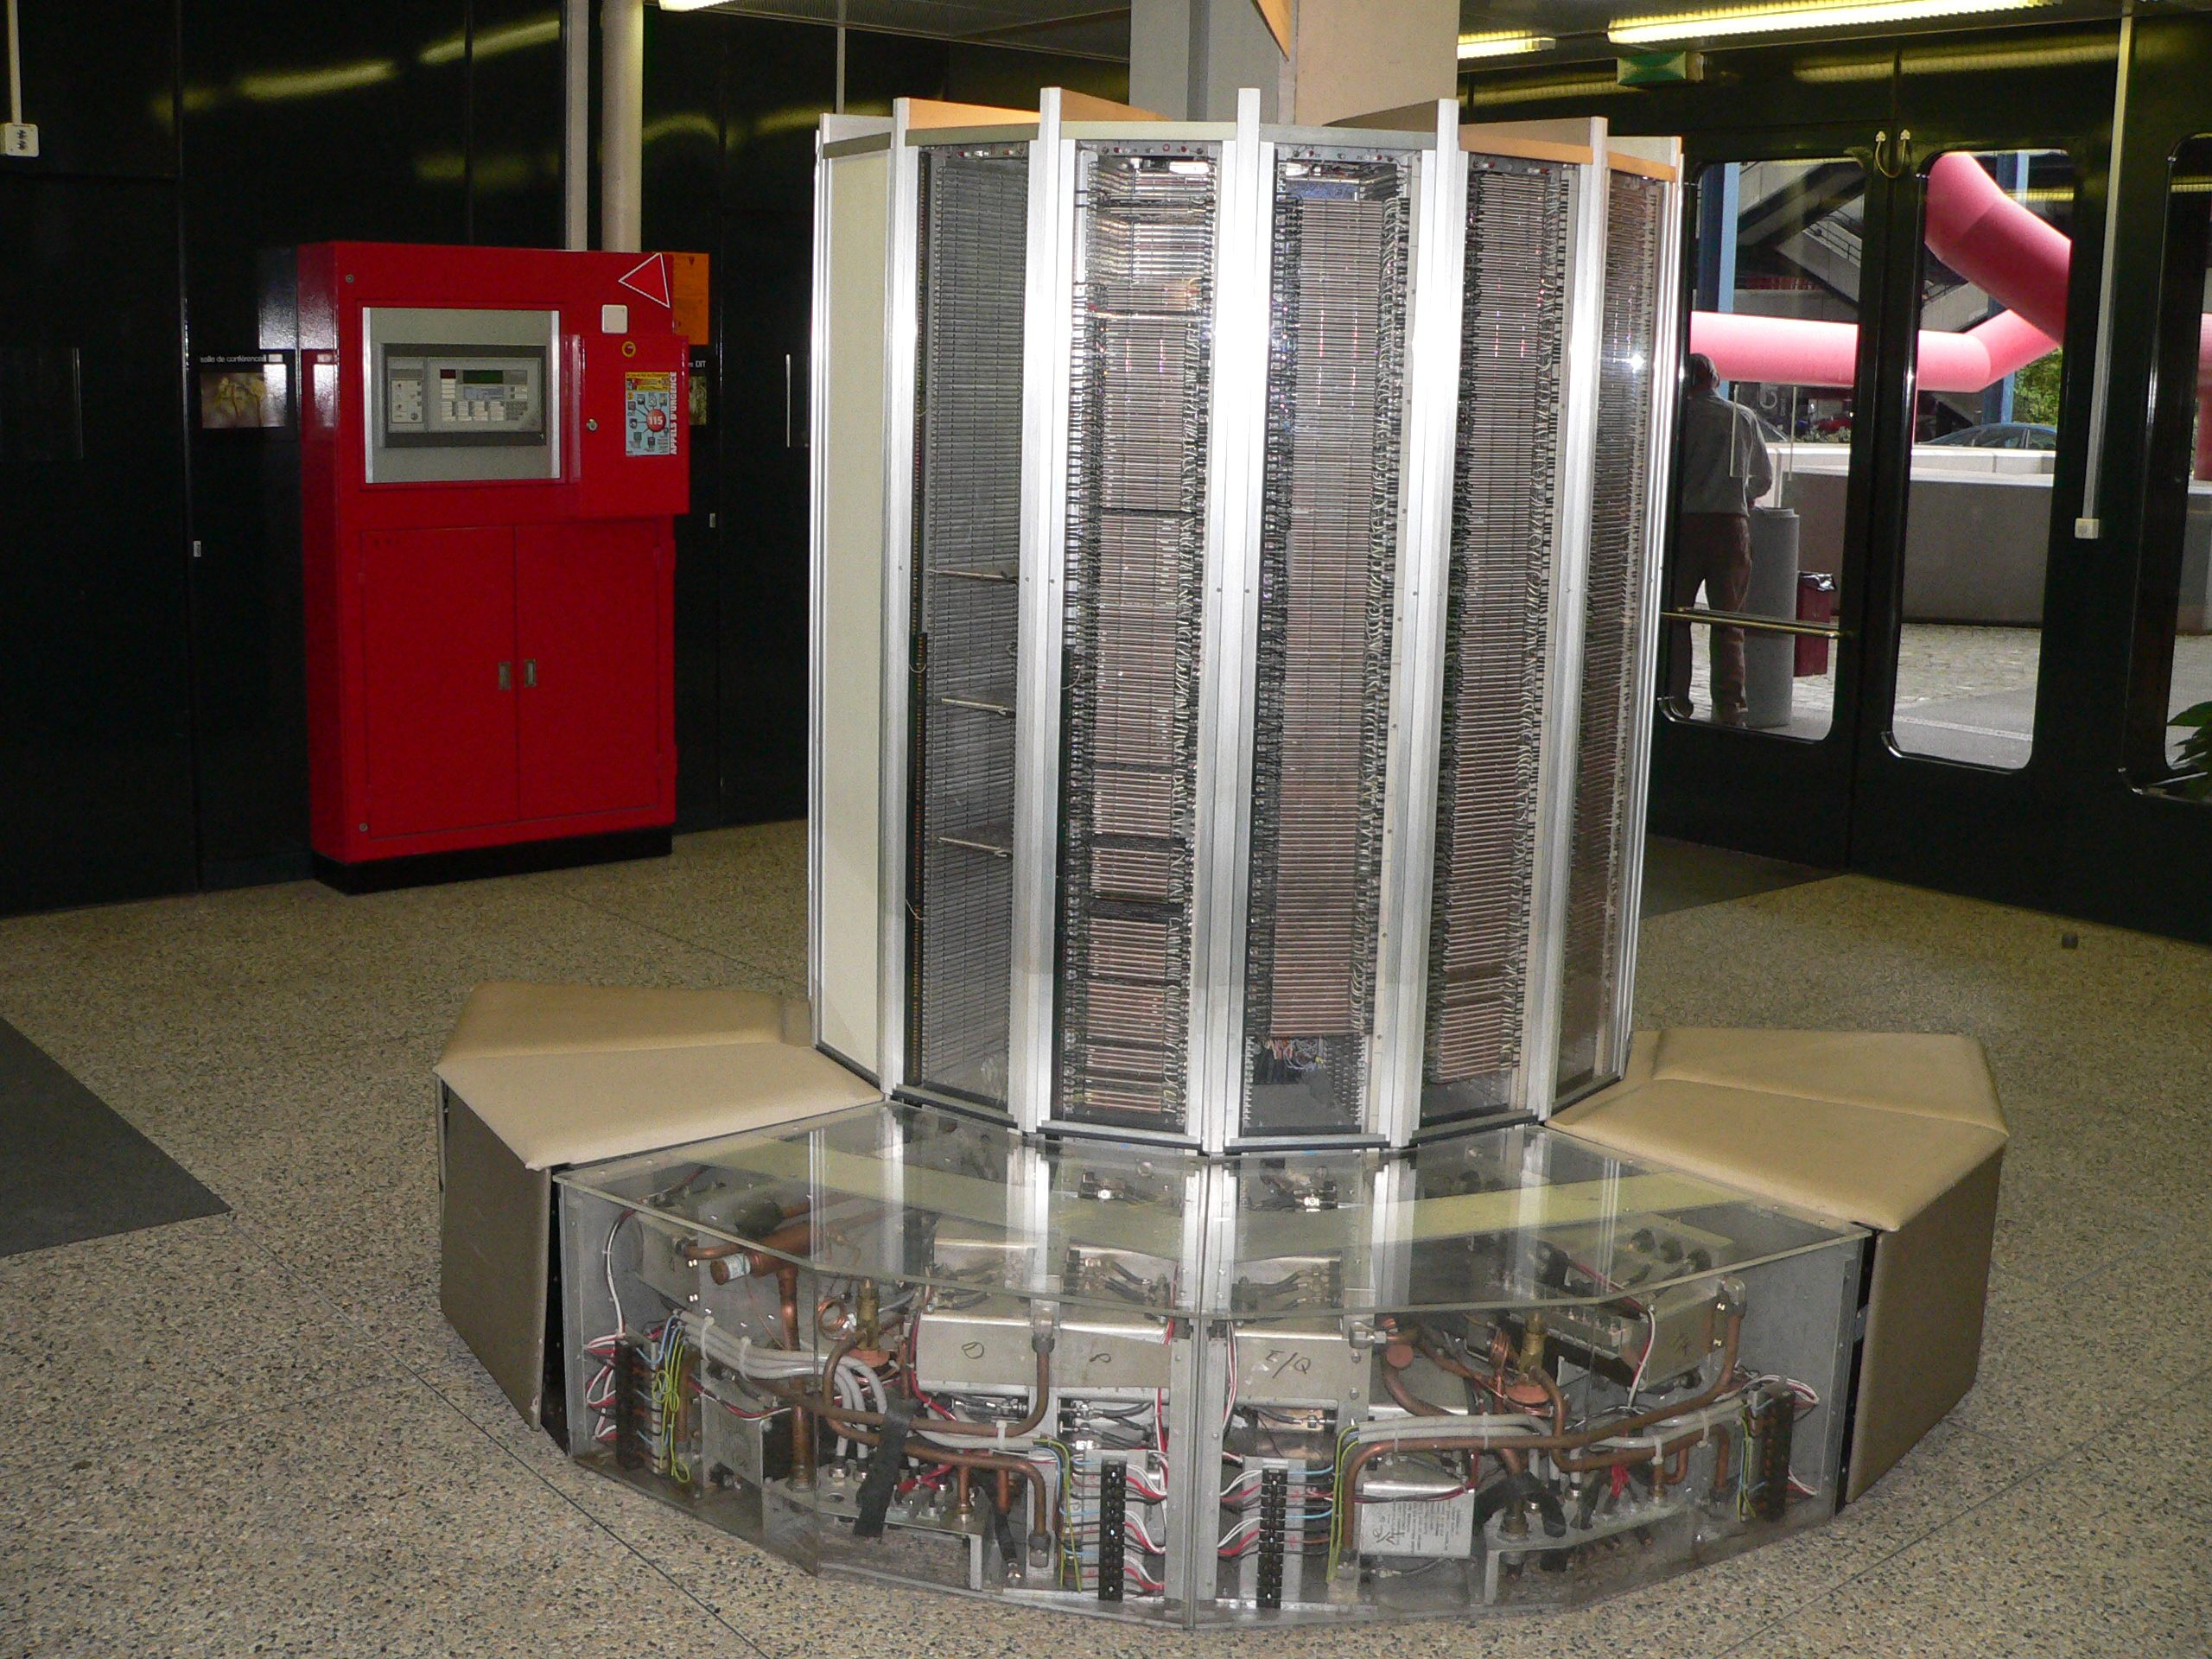
\includegraphics[height=0.3\textheight]{cray.eps}
  \hspace{0.01\textwidth}
  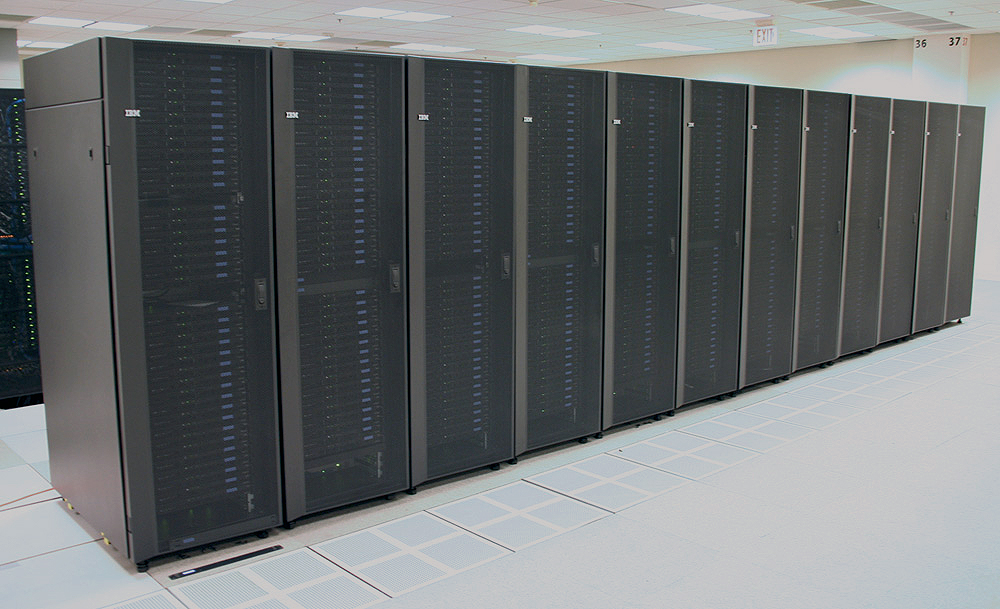
\includegraphics[height=0.3\textheight]{oscglenn.eps}
  \hspace{0.01\textwidth}
  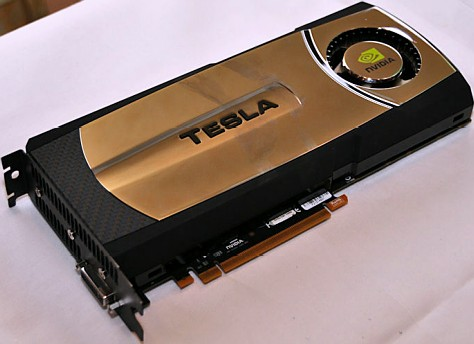
\includegraphics[height=0.3\textheight]{tesla_g300.eps}
\end{center}
\begin{itemize}
  \item 1970-1990: Vector machines (Cray computers).
  \item 1990-200x: Clusters with MPI.
  \item Now: Many-core technology, e.g., general-purpose GPU clusters.
\end{itemize}
\end{frame}

\begin{frame}{
%
Hybrid Parallel Computing
%
}
\begin{minipage}[c]{\textwidth}\centering
\parbox{0.3\textwidth}{\centering
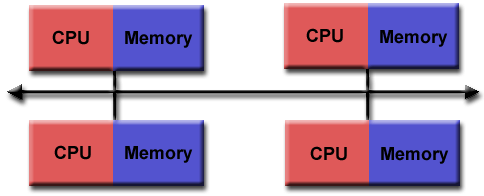
\includegraphics[width=0.3\textwidth]{mem_distributed.eps} \\ distributed
(cluster)}
+ 
\parbox{0.3\textwidth}{\centering 
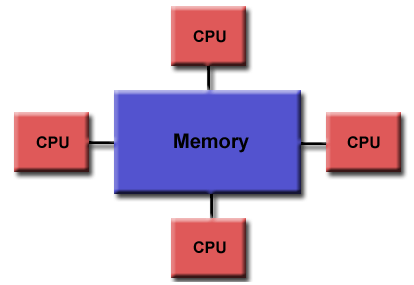
\includegraphics[width=0.3\textwidth]{mem_shared.eps} \\ shared (vector/GPU)}
= 
\parbox{0.3\textwidth}{\centering
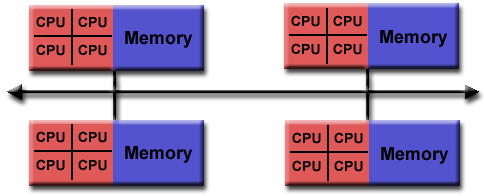
\includegraphics[width=0.3\textwidth]{mem_hybrid.eps} \\ hybrid (GPU cluster)}
\end{minipage}
\begin{itemize}
  \item Definition: Simultaneously use distributed-memory (e.g., MPI) and
  shared-memory (e.g., CUDA/OpenCL) parallel computing.
  \begin{itemize}
    \item The difference in parallel computing models requires using disparate
    programming tools.
  \end{itemize}
  \item Software structure needs to be organized to accommodate the different
  computing models.
\end{itemize}
\end{frame}

\begin{frame}{
%
Python Addresses the Challenges in HPC
%
} \large
\begin{itemize}
  \item Three challenges for the next-generation solvers of hyperbolic PDEs.
  \begin{itemize} \large
    \item \alert{Challenge 1}: HPC by using advanced hardware, e.g., GPGPU
    computing, CUDA/OpenCL, hybrid parallelism, etc.
    \item \alert{Challenge 2}: I/O and post-processing large data; the
    bottleneck is the laborious work flow for post-processing the results.
    \item \alert{Challenge 3}: Code reuse for long life cycle: Extend the
    technologies for various applications.
  \end{itemize}
  \item Python can address the challenges.
  \begin{itemize} \large
    \item SOLVCON is a successful prototype.
    \item NumPy is the foundation.
  \end{itemize}
\end{itemize}
\end{frame}

\section{Conclusions}

\begin{frame}{
%
Conclusions
%
}
\begin{itemize}
  \item De facto Python tool chain for scientific/engineering computing: NumPy
  + SciPy + Matplotlib.
\end{itemize}
\end{frame}

\end{document}

% vim: set spell:
